% ============================ Part 5: RL basics ============================
\section{Part 5 $\cdot$ RL basics}
\partslide{5}{RL basics}{learning from a score instead of a label}

\begin{frame}{Reinforcement learning in one picture}
\begin{columns}[T]
\begin{column}{0.46\textwidth}
\centering
\begin{tikzpicture}[font=\small,>=Latex]
  \node[draw,rounded corners,fill=uvanavy!12,minimum width=3.2cm,minimum height=0.9cm,thick] (ag) at (0,0) {\textbf{Agent} (policy $\pi_\theta$)};
  \node[draw,rounded corners,fill=softgray,minimum width=3.2cm,minimum height=0.9cm,thick] (env) at (0,-2.4) {\textbf{Environment}};
  \draw[->,thick] (ag.east) -- ++(1.1,0) -- ++(0,-2.4) -- (env.east);
  \node[right,font=\scriptsize,align=left] at (1.15,-1.2) {action $a_t$};
  \draw[->,thick] (env.west) -- ++(-1.1,0) -- ++(0,2.4) -- (ag.west);
  \node[left,font=\scriptsize,align=right] at (-1.15,-1.2) {state $s_{t+1}$\\reward $r_{t+1}$};
\end{tikzpicture}\\[4pt]
\scriptsize The agent--environment loop (Sutton \& Barto).
\end{column}
\begin{column}{0.52\textwidth}
\begin{itemize}\setlength{\itemsep}{5pt}
  \item \textbf{State $s_t$:} what the agent observes; \textbf{action $a_t$:} what it does.
  \item \textbf{Reward $r_t$:} a number from the environment. It is the \emc{only} feedback the agent gets.
  \item \textbf{Policy $\pi_\theta(a\mid s)$:} a distribution over actions given the state. In other words, \emc{a classifier again}.
  \item \textbf{Goal:} maximize the expected total reward $J(\theta) = \E_{\pi_\theta}\big[\sum_t r_t\big]$.
\end{itemize}
\end{column}
\end{columns}
\vspace{6pt}
\keybox{Examples: Atari and Go (reward = score, win), a walking robot (distance), \dots\ and a chatbot?}
\end{frame}

\begin{frame}{Supervised learning vs.\ reinforcement learning}
\centering
\renewcommand{\arraystretch}{1.35}\setlength{\tabcolsep}{4pt}
\begin{tabular}{@{}p{2.2cm}p{5.1cm}p{5.9cm}@{}}
\toprule
 & \textbf{supervised learning} (so far) & \textbf{reinforcement learning}\\
\midrule
feedback & the \emph{correct output} $y^\star$ for each input & only a \emph{score} $r$ for the output you produced\\
data & fixed dataset, i.i.d. & generated by \emph{your own} policy, so it changes as you learn\\
granularity & per example, per token & often one number at the \emph{end} of a long sequence\\
objective & minimize loss against labels & maximize expected reward\\
hard parts & (none of these) & \textbf{exploration}, \textbf{credit assignment}, \textbf{instability}, etc.\\
\bottomrule
\end{tabular}
\vspace{10pt}

\keybox{Why bother? For ``is this helpful?'' or ``is this proof correct?'', a \textbf{score} is far cheaper than a \textbf{demonstration}.}
\end{frame}

\begin{frame}{The LLM as a policy}
\begin{columns}[T]
\begin{column}{0.55\textwidth}
\begin{itemize}\setlength{\itemsep}{5pt}
  \item \textbf{State $s_t$} = (prompt $x$, tokens generated so far $y_{<t}$)
  \item \textbf{Action $a_t$} = the next token $y_t\in V$
  \item \textbf{Policy} $\pi_\theta(a_t\mid s_t) = p_\theta(y_t\mid x, y_{<t})$, the same softmax classifier as in language modeling
  \item \textbf{Episode} = one complete response $y = (y_1,\dots,y_T)$
  \item \textbf{Reward} $R(x,y)$ = a score for the \emc{whole} response, given once at the end
\end{itemize}
\end{column}
\begin{column}{0.43\textwidth}
\centering
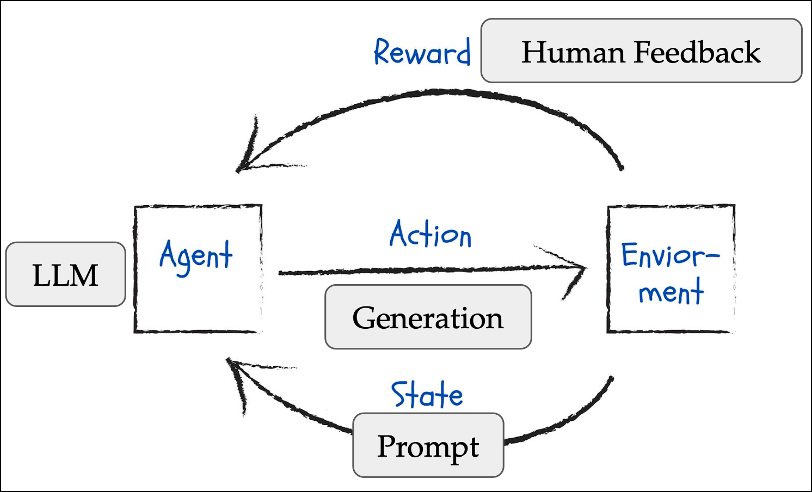
\includegraphics[width=0.9\textwidth]{figs/alignment_as_rl.png}\\[2pt]
\scriptsize Prompt = state, generation = action, feedback = reward.
\end{column}
\end{columns}
\vspace{4pt}
\keybox{\textbf{Objective:} \; $J(\theta) = \E_{x\sim\mathcal{D}}\,\E_{y\sim\pi_\theta(\cdot\mid x)}\big[R(x,y)\big]$\\[3pt]
\small Where does $R$ come from? Either a \textbf{reward model} learned from human preferences (RLHF), or a \textbf{program} that checks the answer (RLVR).}
\end{frame}

\begin{frame}{Policy gradient: how to increase a reward you can only sample}
Goal: maximize $J(\theta)=\sum_y \pi_\theta(y\mid x)\,R(x,y)$. We cannot differentiate $R$ (a human judgment, a checker), but we can differentiate $\pi_\theta$:
\begin{align*}
  \nabla_\theta J(\theta) &= \sum_y \nabla_\theta \pi_\theta(y\mid x)\, R(x,y) && \text{\small\color{midgray} $R$ does not depend on $\theta$}\\
  &= \sum_y \pi_\theta(y\mid x)\, \nabla_\theta \log \pi_\theta(y\mid x)\, R(x,y) && \text{\small\color{midgray} because $\nabla \pi = \pi\,\nabla\log\pi$}\\
  &= \E_{y\sim\pi_\theta(\cdot\mid x)}\Big[\, R(x,y)\; \nabla_\theta \log \pi_\theta(y\mid x) \,\Big] && \text{\small\color{midgray} an expectation: estimate it with samples}
\end{align*}
\vspace{-4pt}
\textbf{REINFORCE} (Williams, 1992): sample a response $y$, then $\;\theta \leftarrow \theta + \alpha\, R(x,y)\, \nabla_\theta \log \pi_\theta(y\mid x)$.
\vspace{-2pt}
\begin{columns}[T]
\begin{column}{0.5\textwidth}
\keybox{\textbf{Why the log?} The sum runs over all $|V|^T$ possible responses. The identity $\nabla\pi=\pi\,\nabla\log\pi$ turns it into an \emc{average over samples} from the current policy.}
\end{column}
\begin{column}{0.48\textwidth}
\keybox{\textbf{And it splits per token:} $\log\pi_\theta(y\mid x)=\sum_t \log p_\theta(y_t\mid x,y_{<t})$. Same form as an SFT step, but on the model's \emc{own sample} $y$, not a label, and weighted by $R$.}
\end{column}
\end{columns}
\end{frame}

\begin{frame}{Read it as: sample $\to$ score $\to$ SFT-shaped step on the sample}
\begin{center}
\renewcommand{\arraystretch}{1.6}
\begin{tabular}{@{}lll@{}}
\toprule
 & \textbf{gradient} & \textbf{where $y$ comes from}\\
\midrule
\textbf{SFT} & $1 \cdot \nabla_\theta \log p_\theta(y^\star\mid x)$ & a \emph{human} wrote $y^\star$ (a label)\\
\textbf{RL} & $\textcolor{uvaorange!85!black}{R(x,y)} \cdot \nabla_\theta \log \pi_\theta(y\mid x)$ & the \emph{model} sampled $y$ (not a label)\\
\bottomrule
\end{tabular}
\end{center}
\vspace{6pt}
\keybox{\textbf{Policy gradient has the same form as an SFT step, but the sequence is the model's own sample and it is weighted by how good that sample was.}}
\vspace{6pt}
\begin{itemize}\setlength{\itemsep}{4pt}
  \item Nothing changes in the network, the softmax head, or the optimizer.
  \item What changes: the data is the model's own output, and each sequence carries a \emc{weight}.
\end{itemize}
\end{frame}

\begin{frame}{Baselines and the advantage: good \emph{relative to what}?}
\begin{columns}[T]
\begin{column}{0.56\textwidth}
\begin{itemize}\setlength{\itemsep}{3pt}
  \item If every response scores $0.6$--$0.9$, \emph{all} get pushed up. Only differences carry information.
  \item Fix: subtract a \textbf{baseline} $b(x)$ that does \emc{not depend on the sampled $y$}:
  \[ \nabla_\theta J = \E\big[(R(x,y) - b(x))\,\nabla_\theta\log\pi_\theta(y\mid x)\big] \]
  \vspace{-10pt}
  \item Still unbiased, since $\E_{y}[\nabla_\theta\log\pi_\theta(y\mid x)] = 0$. A \emc{well-chosen} $b$ (near the expected reward) cuts the variance a lot; a poor one can even raise it.
  \item \textbf{Advantage} $A = R - b$: ``how much better than expected''.
  \item $b$: a learned value function (``critic'') in classic RL; a \emc{group of samples} in GRPO.
\end{itemize}
\end{column}
\begin{column}{0.42\textwidth}
\centering
\begin{tikzpicture}
\begin{axis}[width=\textwidth,height=4.2cm,ybar,/pgf/bar width=10pt,ymin=0,ymax=0.5,
  symbolic x coords={$y_1$,$y_2$,$y_3$,$y_4$},xtick=data,ylabel={$\pi_\theta(y\mid x)$},ylabel style={font=\scriptsize},
  yticklabel style={font=\tiny},xticklabel style={font=\scriptsize},enlarge x limits=0.18,title={advantage $A=R-b$: push mass toward $A>0$},title style={font=\scriptsize}]
\addplot[fill=uvanavy!40,draw=uvanavy] coordinates {($y_1$,0.30) ($y_2$,0.25) ($y_3$,0.25) ($y_4$,0.20)};
\node[above,font=\scriptsize,text=okgreen!70!black] at (axis cs:$y_1$,0.30) {${+}0.5\ \uparrow$};
\node[above,font=\scriptsize,text=badred] at (axis cs:$y_2$,0.25) {${-}0.3\ \downarrow$};
\node[above,font=\scriptsize,text=okgreen!70!black] at (axis cs:$y_3$,0.25) {${+}0.2\ \uparrow$};
\node[above,font=\scriptsize,text=badred] at (axis cs:$y_4$,0.20) {${-}0.4\ \downarrow$};
\end{axis}
\end{tikzpicture}\\
\scriptsize Four sampled responses to one prompt, rewards $0.9, 0.1, 0.6, 0.0$, baseline $b = 0.4$.
\end{column}
\end{columns}
\end{frame}

\begin{frame}{Stability trick 1: don't move too far in one step (PPO clipping)}
\begin{columns}[T]
\begin{column}{0.55\textwidth}
\begin{itemize}\setlength{\itemsep}{6pt}
  \item The policy \emph{generates its own training data}: one step too far $\to$ garbage samples $\to$ worse step. (In supervised learning the next batch corrects a bad step.)
  \item \textbf{PPO} (2017): per token, let $\rho_t = \dfrac{\pi_\theta(y_t\mid\cdot)}{\pi_{\text{old}}(y_t\mid\cdot)}$ and optimize
  \[ \min\big(\rho_t A,\; \mathrm{clip}(\rho_t, 1-\epsilon, 1+\epsilon)\,A\big). \]
  \item Once a token's probability has moved by $\pm\epsilon$ (e.g.\ 20\%), it gets no further push this round.
\end{itemize}
\end{column}
\begin{column}{0.43\textwidth}
\centering
\begin{tikzpicture}
\begin{axis}[width=\textwidth,height=4.6cm,xmin=0.4,xmax=1.6,ymin=-1.5,ymax=1.5,xlabel={ratio $\rho_t$},ylabel={objective},
  xlabel style={font=\scriptsize},ylabel style={font=\scriptsize},ticklabel style={font=\tiny},xtick={0.8,1,1.2},xticklabels={$1{-}\epsilon$,$1$,$1{+}\epsilon$},
  legend style={font=\tiny,at={(0.03,0.97)},anchor=north west,draw=none,fill=none},axis lines=left]
\addplot[okgreen!70!black,thick] coordinates {(0.4,0.4) (1.2,1.2) (1.6,1.2)}; \addlegendentry{$A>0$: capped above}
\addplot[badred,thick] coordinates {(0.4,-0.8) (0.8,-0.8) (1.6,-1.6)}; \addlegendentry{$A<0$: capped below}
\addplot[only marks,mark=*,mark size=1.5pt,black] coordinates {(1,1) (1,-1)};
\end{axis}
\end{tikzpicture}\\
\scriptsize PPO's clipped objective for one token ($|A|=1$).
\end{column}
\end{columns}
\end{frame}

\begin{frame}{Stability trick 2: stay close to where you started (KL penalty)}
\begin{itemize}\setlength{\itemsep}{8pt}
  \item Subtract a penalty for drifting away from a frozen \textbf{reference model} $\pi_{\text{ref}}$ (usually the SFT model):
  \[
    \max_\theta\; \E_{y\sim\pi_\theta}\big[R(x,y)\big] \;-\; \beta\,\mathrm{KL}\big(\pi_\theta(\cdot\mid x)\,\|\,\pi_{\text{ref}}(\cdot\mid x)\big)
  \]
  \item Keeps the language fluent, prevents collapsing onto one answer, and limits exploiting flaws in the reward.
  \item $\beta$ trades off ``get more reward'' against ``stay a normal language model''.
\end{itemize}
\vspace{10pt}
\callback{regularization}{$L_2$ keeps the weights $w$ near $0$; the KL term keeps the \emph{policy} $\pi_\theta$ near $\pi_{\text{ref}}$. Same idea, different space.}
\end{frame}
